\documentclass[12pt,a4paper]{article}
\usepackage{times}
\usepackage{durhampaper}
\usepackage{harvard}
\usepackage{underscore}
\usepackage{graphicx}
\usepackage{caption}
\usepackage{subcaption}
\usepackage{url}
\usepackage{hyperref}
\usepackage[subtle]{savetrees}
\usepackage[ruled,vlined,linesnumbered]{algorithm2e}
\usepackage{etoolbox}
\patchcmd\thebibliography
 {\labelsep}
 {\labelsep\itemsep=2pt\relax}
 {}
 {\typeout{Couldn't patch the command}}

\citationmode{abbr}
\bibliographystyle{agsm}

\title{Procedural World Building in Roguelike Games}
\author{Benjamin Jones}
\student{Benjamin Jones}
\supervisor{Dr Tom Friedetzky}
\degree{MSci Natural Sciences}

\date{}

\begin{document}

\maketitle

\begin{abstract}

{\bf Context/Background}

Procedural content generation in videogames has seen a surge in popularity in recent years \cite{Hendrikx}. However as game development progress, users expect more and more intelligent and engaging game level design and as a result, investigating new, interesting methods of procedural content generation is vital to keeping end users satisfied.

{\bf Aims}

This project aims to draw comparisons between current methods of procedural content generation in a roguelike game environment and build upon them to create different and exciting methods of level design. The implementation focusses on creating a number of novel algorithms alongside an intelligent method of evaluating their suitability. 

{\bf Method}

A variety of algorithms have be developed and implemented by building on and combining various existing methods found in existing roguelikes and more sophisticated modern games. The fractal diamond-square algorithm is used to generate pseudo-random noise, which is then smoothed out by a customised version of the \emph{Cellular Automata} approach to produce a variety of different overworld environments. Caves are also generated using binary white noise and hybridising these with geometric `space-filling curves' such as the Hilbert curve. The effectiveness of these is then evaluated by a custom heuristic, ensuring the quality of a resulting world. 

% {\bf Proposed Solution}

% The proposed game will be built and played in Java using the \emph{JFrame} and \emph{asciipanel} libraries as a framework. The combination of existing algorithms and novel techniques will produce multiple potential procedurally generated worlds, which will be evaluated by the program and the best fit will form the playable environment in a roguelike game. 


{\bf Results}

Our new method of generating cave-like structures using geometric curves produces diverse, `interesting' caves, generating paths that the player is able to follow without realising a fixed geometric structure exists. Our method of generating overworld environments based on the diamond-square algorithm is also capable of generating aesthetically fantastic and natural worlds very efficiently. The world evaluation heuristic, while performing adequately in order to prove the concept of post-production evaluation, has room for improvement.

{\bf Conclusion}

The techniques described in this work, although in their infancy, display excellent promise. We show that both the Cellular Automata algorithm and diamond-square algorithm are viable candidates for future roguelikes, and present a new technique for generating cave-like structures that is capable of bridging the gap between traditional, manual methods of content creation with their procedural counterparts. 

[TOO happy/colloquial?]

\end{abstract}

% \begin{abstract}
% These instructions give you guidelines for preparing the final paper.  DO NOT change any settings, such as margins and font sizes.  Just use this as a template and modify the contents into your final paper.  Do not cite references in the abstract.

% The abstract must be a Structured Abstract with the headings {\bf Context/Background}, {\bf Aims}, {\bf Method}, {\bf Results}, and {\bf Conclusions}.  This section should not be longer than half of a page, and having no more than one or two sentences under each heading is advised.
% \end{abstract}

\begin{keywords}
Procedural content generation, roguelike, world building, noise algorithms, artificial intelligence, heuristic, space-filling algorithms.
\end{keywords}

\section{Introduction}


\subsection{Roguelike Games}

The term \emph{roguelike} stems from the original 1980s UNIX dungeon crawler \emph{Rogue} created by Michael Toy and Glenn Wichman, giving birth to hundreds of games such as \emph{Nethack} and \emph{Dwarf Fortress} that follow the same style and structure and revolutionising the gaming industry as we know it today \cite{Dunhack}. There are many different styles of roguelikes these days, but most share the same core features: turn-based gameplay, procedurally generated tile-based dungeons or maps, and randomly created monsters and items \cite{pgcbook}. 


The basic premise of the game has the player controlling a single character through numerous ASCII represented areas filled with monsters, items and traps. However what made it so revolutionary at the time was the fact that the game was different (and the gameplay unique), every time you played it thanks to its procedurally generated nature and random seeds, and its ability to create millions of unique playable dungeons was unparalleled \cite{platformgames}. However these days players expect more from games and we aim to advance on the relatively basic types of procedural generation seen in these early fan favourites. 


This work aims to investigate existing methods of procedural generation within videogames and create a new approach that is both visually appealing and interesting to play to meet the increasing demands of the modern gamer. The genre of roguelike games provides an excellent framework for this aim, combining sufficient complexity with an appropriate method of visualisation of the algorithms. We should like to point out that our methods and findings are relevant to applications in other related domains as well.  


% other types of roguelike can be discussed in the previous work area

% Diablo, spore

\subsection{Procedural Content Generation}

Procedural content generation (PCG) is the process of creating content through the use of random (or pseudo-random) numbers as seeds to generate objects using algorithms and mathematical functions, as opposed to the typical method of being manually created by a developer \cite{pgcbook}. This has many possible applications, from running real-world simulations on procedurally generated objects and environments \cite{VAST}, to generating interesting and unique textures and graphics \cite{imagesynth}, and of course for use in video games. In terrain generation and world building, this is often achieved by modifying the results of mathematical noise algorithms \cite{pgcbookch4}, which generate heightmaps or intensity maps that can be adapted to create procedurally generated content, such as terrains or graphics \cite{improvepnoise}.  


Procedural generation has many advantages unrivalled by other generation methods: it has the ability to generate arbitrarily complex and intricate designs on-the-fly, takes up less storage and has a particularly low memory footprint \cite{surveyPNF}. Additionally, the variation of input parameters can easily generate an incredible number of uniquely styled designs. The result is that procedurally generated game content has the capability to offer every game user a unique gaming experience every time they play. 

% One of the most advanced examples of PCG in roguelikes to date is Bay12Games's 2006 creation Dwarf Fortress. 

As games get more complex and take longer to build, coming up with new and exciting ways to programatically generate game content could be the key to a revolution a game industry expected to reach \$103bn in 2017 \cite{newzoo}. Furthermore, as the industry continues to get more and more competitive, procedural generation is likely to play a key role in allowing indie game developers to keep up with their big-budget counterparts.

\subsection{Contribution Direction}

While roguelikes and their derivatives remain popular more than 40 years after their introduction, current favourites such as \emph{Nethack} and \emph{Dwarf Fortress} struggle to bridge the gap between being visually appealing and functionally engaging. While \emph{Nethack} offers intricate and complex gameplay mechanics, its level design is basic and while more recent editions have offered a graphical tile-based experience, there is still an argument for increasing the graphical capabilities of roguelike games to keep up with the modern market. On the other hand, \emph{Dwarf Fortress} offers incredibly complex algorithmic techniques (owing to its 10 years of alpha-phase development), but again falls short in visual aesthetics. 

This work aims to expand on existing procedural generation techniques in roguelike games, intending to create worlds in a roguelike setting that are both visually pleasing to the modern gamer whilst maintaining the complexity and gameplay aspects that have enticed thousands of players over the years. We predicted that successful implementations of procedural content generation, both in roguelikes and in a wider context, have the ability to satisfy gamers while reducing the cost of content creation significantly, as well as increasing entertainment and replayablility. The latter not only has important implications in the well established single-player market, but also in the expansive domain of massively multiplayer online games (MMOGs), most of which gain revenue from the continued and repeated involvement of players month to month, and estimated to lead the global games market in 2018 with a predicted revenue of approximately \$34.3bn \cite{newzoo}. 



\begin{figure}
\centering
\begin{subfigure}{.5\textwidth}
  \centering
  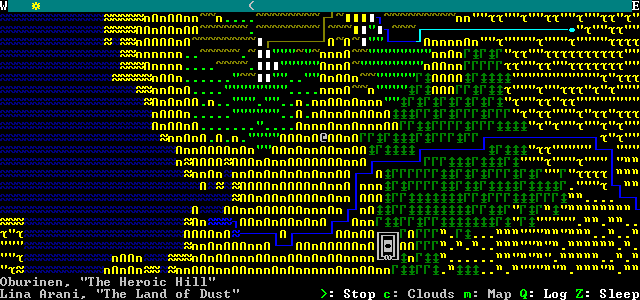
\includegraphics[width=.6\linewidth, height=3cm]{images/dwarffortress.png}
  \caption{A sample of the playable overworld in \emph{Dwarf Fortress}.}
  	\caption*{\small Image sourced from: \url{www.bay12games.com}}
  \label{fig:sub1}
\end{subfigure}%
\begin{subfigure}{.5\textwidth}
  \centering
  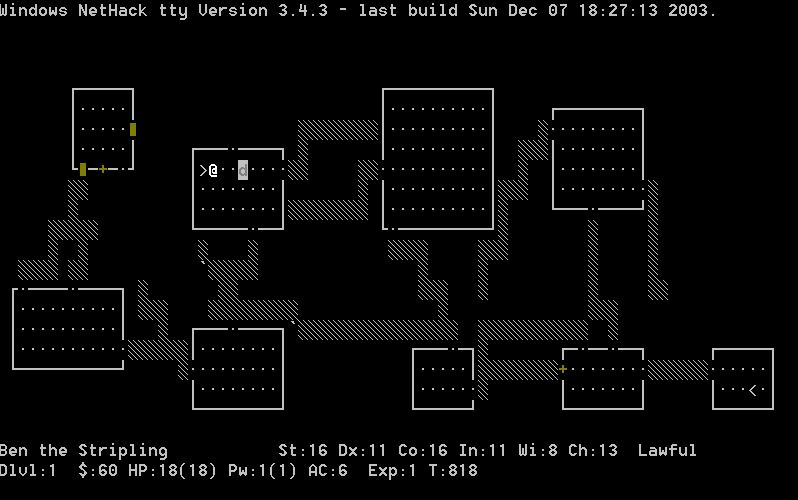
\includegraphics[width=.6\linewidth, height=3cm]{images/nethack3.png}
  \caption{Typical generated dungeon structure in \emph{Nethack}.}
  \label{fig:sub2}
  \ \\
  \ \\
\end{subfigure}
\caption{Comparison of popular roguelike world representations.}
\label{fig:1}
\end{figure}


% \begin{figure}
% \centering
%  	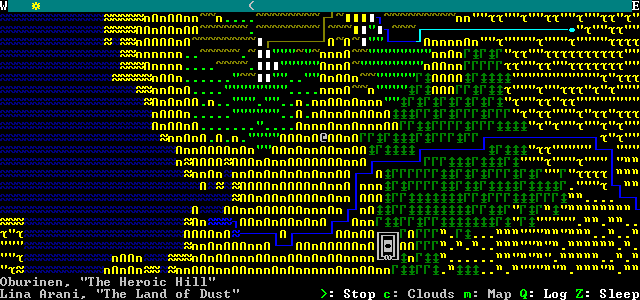
\includegraphics[width=6.25cm,height=4cm]{images/dwarffortress.png}
% 	\caption[]{A sample of the playable overworld in \emph{Dwarf Fortress}. Image sourced from: \url{http://www.bay12games.com}}
% 	\label{fig:fig1}
% 	\vspace{2ex}
% 	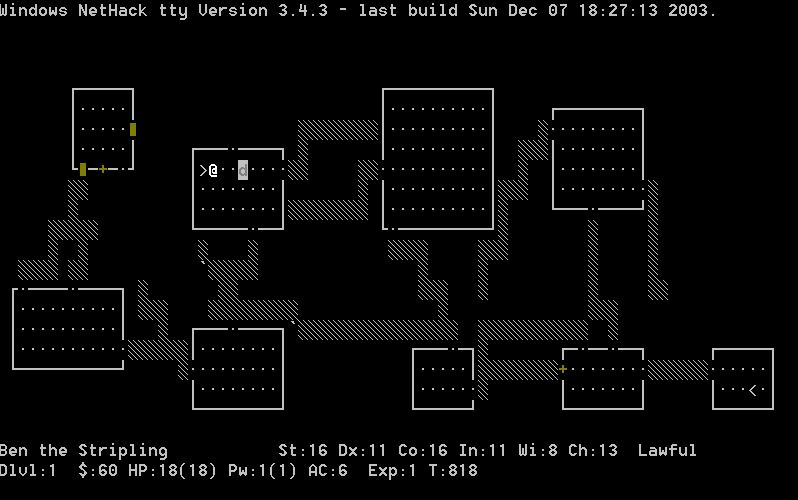
\includegraphics[width=6.25cm, height=4cm]{images/nethack3.png}
%   \caption[]{Typical generated dungeon structure in \emph{Nethack}.}
%   \label{fig:fig2}
% \end{figure}


\subsection{Deliverables}

The purpose of this work in summary was to investigate the various ways in which procedural content generation is used to generate game environments, and then design and build one or more variants based on the best of these approaches with the intent to create exciting and visually interesting in-game environments in a roguelike design space. The algorithm also intended to analyse created worlds to evaluate a measure of how interesting a world is, and only produce worlds that pass a set threshold to the player. Please note unfamiliar concepts in this section will be discussed in greater detail in section \ref{solutions}.

In order to achieve this, the project was split into basic, intermediate and advanced deliverables. The basic objective intended to produce a Java executable capable of handling user input, and output an ASCII grid output, providing a platform to display 2D ASCII environments for a player to explore indicative of the roguelike genre. The world generation algorithm was to be probabilistic and include a 2D noise generator, providing the fundamental basis for procedural environment generation. The algorithm was then to provide a method of 2D noise smoothing, with the smoothing function able to produce explorable areas and structures for a player to explore. 

We achieved the basic objective with an implementation in Java using the AsciiPanel library to produce a graphical user interface (GUI) to provide input and output to the player. A basic noise function of binary random output was created, and a smoothing function based on the \emph{Cellular Automata} ruleset was applied to form arbitrarily sized `caves' from the noise, explorable by a player.

The intermediate objectives were focussed on enhancing the in-game environment by implementing a more complex heightmap noise algorithm capable of producing more realistic in-game environments that exhibit contour behaviour, whereby the noise in one location is dependant on the surrounding elevation, mimicking the gradient nature of real-world environments. A further criteria was the that the generation algorithm was capable of operating efficiently, such that worlds could be evaluated based on a `variability' heuristic and then re-drawn instantaneously or even multiple times should a map not reach the thresholds set.


These intermediate objectives were achieved after researching various different noise algorithms. In the end, the fractal \emph{diamond-square} algorithm was adopted due its capability to produce contour based continuous heightmaps with low memory and CPU overheads, making it perfect for a roguelike game. This was then combined with a custom-made variant of the \emph{Cellular Automata} algorithm to smooth the noise, producing worlds that match the criteria to create more realistic worlds. Furthermore the efficient method of this noise generation and smoothing approach means that the variability coefficient- calculated by statistical analysis of the generated heightmap- can be used to evaluate worlds and regenerate worlds  on-the-fly that do not match up to the variability criteria set in order to make a world `interesting'. 

The advanced criteria for this work was that worlds created should have `distinctive' features, and that worlds would be distinguishable on each playthrough to create a unique gaming experience that worked so well in \emph{Rogue} and subsequent derivatives. An extension to this includes the use of underlying mathematical functions, space-filling curves, that should exist within the structure of the heightmap to decrease the likelihood of encountering `dead ends' within game structures and increase player enjoyment.  Another aspect of the advanced criteria was that algorithm should also be able to identify connected regions of the map, with an understanding of how connected the produced environment is.

One of the advantages of procedural generation over traditional content production is the ability to create vastly different environments with minimal effort. We demonstrated this capability with the introduction of an overworld with a customisable probability function, allowing the developer to create a variety of different \emph{biomes} by adapting the heightmap transformation probabilities. Furthermore, we introduced the ability to feed in distinctive world features such as the \emph{Hilbert} space-filling curve to the noise generation algorithm, adding an underlying structure to the caves that are prevalent throughout the overworld. Finally, a breadth first \emph{flood-fill} search algorithm was used to identify connected regions of the map from the players position. 


\section{Related Work}

In this section it is critical that we survey a range of examples of different procedural generation techniques and how they are used in order to gain a deeper insight into current relevant work. However, it is important to note that due to the nature of the project content, related work comes from many sources including big-budget commercial gaming developers, academic researchers and a large active community roguelike enthusiasts; the latter of which have discovered a wealth of techniques that may be relevant and should not be overlooked, but instead critically evaluated for their individual contributions to the field.

A perfect example of the power and potential of PCG is \emph{Minecraft}. At the time of writing, \emph{Minecraft} sales have hit more than 70 million world-wide, making it one of the most popular games of all time \cite{ukie}. However at its base, \emph{Minecraft} draws many parallels with the methods of generation seen in even some of the earliest roguelike games; for example it uses at its core a 3D adoption of the 2D Perlin fractal noise algorithm adopted by many popular roguelikes \cite{notch}, including the 2006 variant, \emph{Dwarf Fortress} \cite{Dunhack}. 

Also recently hitting the spotlights is indie game \emph{No Man's Sky}, a futuristic sci-fi role-playing game (RPG) that procedurally generates an entire universe populated with up to 18 quintillion planets for the player to explore at their leisure \cite{E3}. Developed by a team of only 10 people, \emph{No Man's Sky} demonstrates the power and potential that procedural generation has to offer to the gaming market. 

Another small budget game worth mentioning is award-winning 2004 German 3D shooter \emph{.kkrieger}. The game won its award not because of its content however, but because of its extensive use of procedural generation techniques mean everything from the textures to the in-game sounds (as well as the traditional monsters and levels) are generated completely procedurally. This allows the entire game to be coded in just 96 kilobytes of memory, meaning that even screenshots of the game take up more room than the game itself- allowing \emph{.kkrieger} to take up 3000x less storage than an equivalent conventionally designed game \cite{kkrieger}. This game exemplifies what can be achieved using procedural techniques. 

--Talk about dwarf fortress/ diablo here. Cant find good source on techniques used by these

The \emph{Diamond-Square} algorithm used in this work was initially proposed by Fournier, Fussell and Carpenter at the SIGGRAPH conference in 1982 and is an efficient way of generating fractal heightmaps in computer graphics \cite{FournierDSq}. It is particularly effective at modelling the contours of natural landscapes and is even used by Planetside Software in their professional scenery generator program \emph{Terragen} \cite{claghorn}, whose outputs can be seen in popular movies such as \emph{Star Trek Nemesis} and \emph{The Golden Compass} \cite{planetside}. 

It is important to point out however that the algorithm is not without its flaws and Gavin S. Miller notes in his 1986 paper \emph{The Definition and Rendering of Terrain Maps} that the algorithm is subject to `the creasing problem', whereby creases and slope discontinuities occur along the boundaries between fractals \cite{GMillerDiamondSq}. He then goes on to suggest a more complex `improved' algorithm based on weighted averages and control points that he suggests overcomes the problems in the original's design. Paul Martz however argues in his article, `Generating Random Fractal Terrain' (1997), that Miller is simply attempting to use the algorithm for the wrong purposes, and goes on to show that if one does not try to `force' peaks to occur in the central array location by generating only positive pseudo-random numbers, the algorithm produces much better results. 

[NOTE: I have these referenced in bibtex but because I don't directly cite them they don't appear in bibliography- how to do this?]

One of this projects aims is to self evaluate generated worlds. While relatively little work in this field exists, Roland van der Linden \emph{et al}. in their work `Procedural Generation of Dungeons', attempt to describe ways in which gameplay-based control, that is the actions of the player, are able to influence the creation of PCG using data collected in-game. They admit however that extending this concept to evaluate how successful newly generated worlds are is still a challenge, and do so by manual feedback checks at the time of writing. 

A more promising example is described by Mahlmann \emph{et al.} in `Spicing Up Map Generation', where the authors describe post-generation evaluation techniques used in the popular strategy game \emph{StarCraft}. Here, they describe how a handful of functions dictate the world production process, including distance and path calculations (such as distances from bases to resources) and multi-objective evolutionary algorithms, which are used to evaluate the interplay between their evaluation criteria. A map that is deemed `good enough' in all relevant dimensions is then provided to the player. The researchers argue however that the evaluative techniques used in StarCraft slow down the map generation process to unacceptable levels, and go on to propose a new method for generating and evaluating maps, using similar concepts to those described above. After assigning appropriate parameters, the team then go on to produce a genetic-style algorithm that generates many maps, testing each for their fitness while recording the most successful parameters from each run. Running their algorithm on maps created by \emph{Dune 2}, the team eventually are able to exclusively recreate `good' worlds. 

The findings from the team look promising, however it should be pointed out that their criteria for a `good enough' world is not particularly stringent in our opinion, and the researchers themselves point out that whether their generated worlds would be deemed `interesting' from a players point of view remains to be seen. 


 Recognising that devising a single good
evaluation function for something as complex as a strategy game map is anything
but easy, the authors defined a handful of functions, mostly based on distance
and path calculations, and used multi-objective evolutionary algorithms to study
the interplay and partial conflict between these evaluation dimensions. While
providing insight into the complex design choices for such maps, it resulted in
a computationally expensive map generation process and problems with finding
maps that are “good enough” in all relevant dimensions. The map representation
is a combination of direct (positions of bases and resources) and indirect (a turtlegraphics-like
representation for rock formations), with mixed results in terms of
evolvability



% Having evaluated his argument however, we feel these negatives are outweighed by its fast evaluation time and impressive results, and are unlikely to become a problem in a roguelike setting. 


% - Talk about image generation of TerraGen - using midpoint displacement 

% - Talk about other relevant examples of the algorithms i use

% - Talk about perlin noise research and why i didnt use that- allude to the negatives of this approach/ scalability. talk about simplex noise also
% 	-- but implementation difficulty and runtime didn't match criteria for advanced objectives of tradeoff for worlds capabale of being produced quickly  

% - Talk about the extended usage of these in minecraft and other things 

% - Hilbert curve research? 

% - Noise generation in amateur games - many references on this in my diss folder 

% - Research into cellular automata? 

% - Could talk about dwarf fortress/ other roguelikes 

% - Canyon 3d work 
% 	- work by M carli et al on canyon creation using mean shift algorithm 
% 	- shows how you can bridge the gap between 2d and 3d, how 2d algorithms are relevant
% 	- explain that an implementation represented in 2d is still a 3-dimensional map just projected into 2d
% 	- k means 





\section{Solution} 
\label{solutions}

\subsection{Specification of Software}

The implementation of this work was developed and produced in Java (SE 1.8). There are a number of reasons why Java was well suited to this work. Java is a well established, high-level language preferred by thousands of amateur and professional game developers alike, and as such there are many previous implementations and libraries specific to roguelikes and procedural content generation from which this work was able to benefit from. By utilising copyright-free libraries and examples from other roguelike enthusiasts a quick prototype framework for the game was implemented and subsequently developed to form the foundation of the back-end of the game. This enabled the focus of the project to be on more important and interesting aspects of the generation algorithms. To this extent, many suitable libraries exist, and this work made particular use of the \emph{JFrame} and \emph{AsciiPanel} libraries, in addition to the \emph{Apache Commons Math} packages existing within the Java framework. \emph{JFrame} is a well known and established library enabling the use of a windowed frame for which the program is able to handle input and output, whereas \emph{AsciiPanel} is described as a `Java Console System Interface', popular among roguelikes and allowing for multi-colour ASCII text character output to the \emph{JFrame} environment. In addition to \emph{AsciiPanel}, the implementation made use of an open source framework developed by the creator of \emph{AsciiPanel}, providing access to the various functions that the \emph{AsciiPanel} library provides while allowing the project to focus on more complex aspects of the procedural generation algorithmic design \cite{trystan}. The capabilities of the resulting game engine allowed for an interactive window of a similar quality to that of established roguelikes such as \emph{Nethack} and even \emph{Dwarf Fortress}

Java is also particularly useful due to its highly object-orientated nature. Since the design aspect of the game can be separated into many parts, it is helpful to be able to abstract and separate each process into different classes, allowing the main focus of the algorithmic side of the project to be apart from the engine handling input and output to the console. This makes development much easier, as well as improving bug fixing and code readability.

In addition, Java is known as a platform-neutral language \cite{java}, meaning the final implementation will be easily run on almost any platform (except mobile) without the need to recompile the source. This is very powerful and allowed for continued development and evaluation from a variety of computers during the project. 

Finally, Java was chosen because of its familiarity. While the project may have benefited from features of other languages (such as the rapid prototyping and clear code style of Python), previous familiarity with Java enables a reduced implementation period in the system development life cycle, allowing more time to be spent on the design, planning and evaluation aspects of the cycle. 


\subsection{Methodology}

The \emph{Agile} software development methodology was used in the project in order to meet its aims. This was selected because we felt that the project would benefit from achieving each functional target in individual rapid sprint cycles, which would then be able to be thoroughly tested for quality between cycles before the next implementation aspect was introduced. We also felt that this enabled a higher degree of freedom than other considered software development approaches (such as the \emph{Waterfall} approach), enabling the constant evaluation of the project at regular intervals.

\subsection{Noise and Smoothing Algorithms}

Noise algorithms form the foundation to most procedurally generated content and feature heavily in this work. The purpose of this section talks through the noise and smoothing algorithms that are used in this work, and discusses how they will be used together to create the foundation of a roguelike world. 


\subsubsection{Cellular Automata}

There are a multitude of different noise algorithms [AS DESCRIBED IN SECTION...], but we start by defining discrete binary `white' noise. White noise is a 2-dimensional array of randomly assigned bits that are independent and theoretically identically distributed from each other \cite{stats}. The noise environment can then be modified by a variety of different approaches to form the basis of the content in procedural games. To generate the noise, we use Java's in-built pseudo-random number generator \emph{Random}, from the `Java.Util' package, seeded using a 13-digit long UNIX timestamp.

The binary noise algorithm is simple and easy to implement, paving the foundation for a smoothing technique known as \emph{Cellular Automata}. This technique came about in the 1970s when British mathematician John Horton Conway devised his evolutionary \emph{Game of Life}, a set of rules that transform an initial state of `cells' into intricate and interesting patterns and designs by the use of 3 rules of state \cite{cellauto}:

\begin{itemize}
	\item Survivals: Every cell with two or three neighbouring cells of the same type survives for the next generation.
	\item Deaths: Each cell with four or more similar neighbours dies (is removed) from overpopulation. Every cell with one neighbour or none dies from isolation.
	\item Births: Each empty cell adjacent to exactly three neighbours--no more, no fewer--is a birth cell. A cell is placed on it at the next move.
\end{itemize}

This process is used upon the result of the binary white noise to `smooth' the landscape by turning areas that are mostly neighbouring walls into walls and areas neighbouring floors into floors, however we have adapted the ruleset in order for the algorithm to converge after a finite number of iterations- namely that cells do not `die' if they are surrounded by similar neighbours, and births are suppressed. Repeating the process over multiple iterations has the effect of smoothing the terrain, eventually converging towards a stable environment. 


\begin{figure}[ht]
  \centering
 	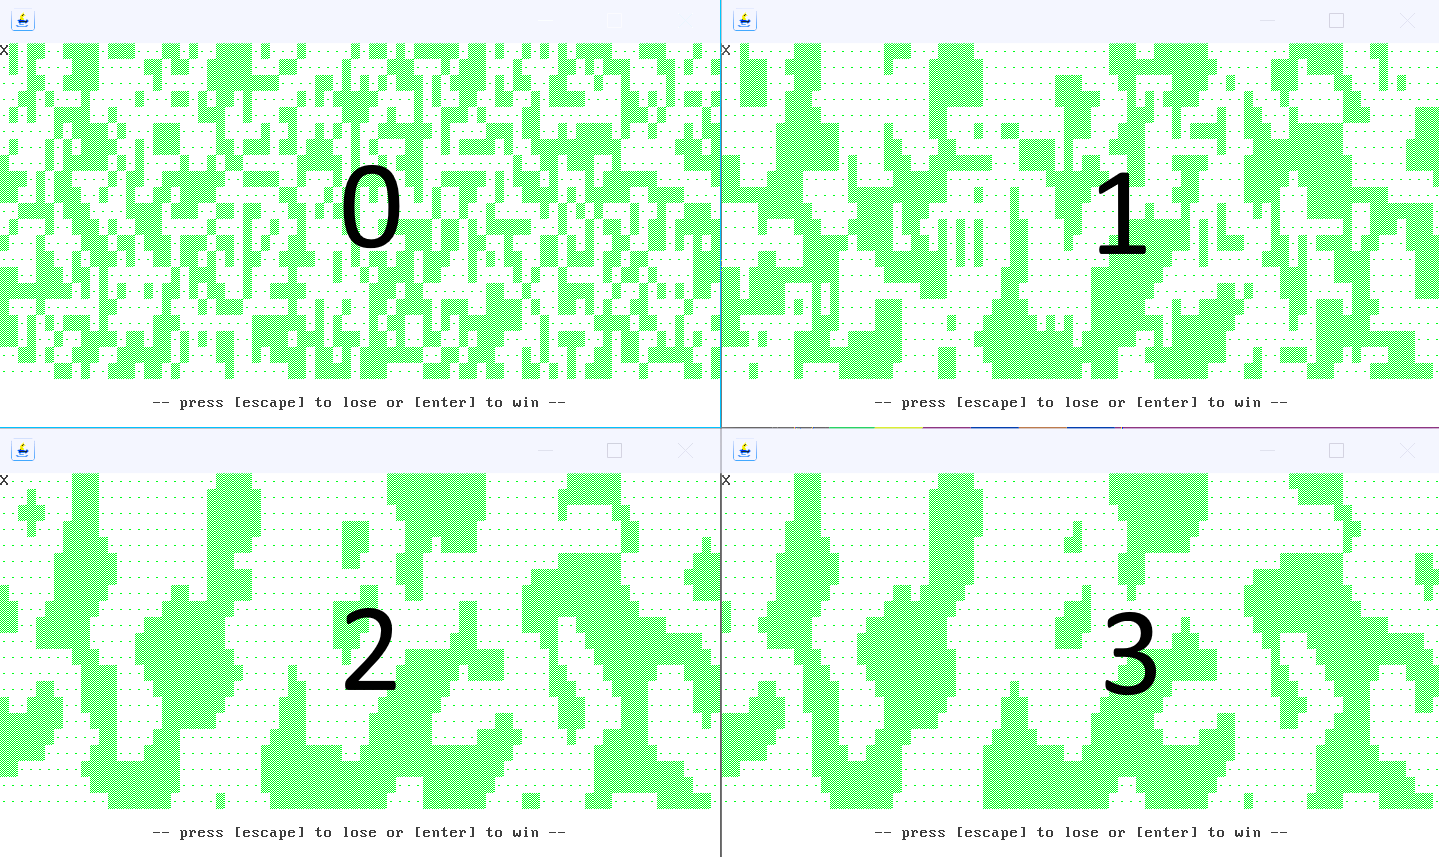
\includegraphics[scale=0.5]{images/cellauto.png}
	\caption[]{Cellular Automata cave smoothing. The numbers indicate the iterations of the algorithm, where the top-left image is before the smoothing process. Image self generated.}
	\label{fig:2}
\end{figure} 

It's clear to see from Figure \ref{fig:2} that this process very quickly converges to produce interesting, procedurally generated cave-like structures for a roguelike game setting, in addition to being computationally inexpensive (the generation is instantaneous even for very high levels of iterations (1000+) on a moderately powerful machine, and has time complexity O($xy$) where $x$ is the width and $y$ is the height of a map \cite{cellularcomplexity}). 

It is, however, limited in its usefulness by itself, as the results of the algorithm are inconsistent, occasionally producing uninteresting or unnatural worlds. Worse still, it is particularly prone to what is known as `the isolated cave problem', whereby produced maps are often particularly `disconnected'- that is the player is often unable to advance to large regions of the cave. 

This nature (seen in Figure \ref{fig:2}) is undesirable in order to fulfil the intermediate aims of the project, and a number of alternative approaches were considered to solve this problem.

One approach for example would be to generate many worlds and test for completeness, discarding the worlds that do not fit our criteria. Because of the instantaneous nature of this method of world population, we are able to create and evaluate many worlds very quickly, however the problem arises when we wish to expand our world size. A larger world boundary results in an increased statistical probability that the created world will be highly disjoint almost every time. An alternative approach would be to identify disjoint sections and post-process connect them up by removing wall segments. This does guarantee connectivity, but is also prone to making the world look `unnatural', defeating the point of using the algorithm in the first place. One of the biggest advantages with \emph{Cellular Automata} however is that rules can be tweaked easily to modify the output to the developers preference, and this is exactly what amateur developers at \emph{RougeBasin} have done \cite{roguebasin}. By experimenting with the probabilities of birth and death rates, they are able to create connected caves that still maintain their natural look and feel.

This solution works well for smaller game environments, however even with the finest tweaking of parameters, its output is still unable to cope with moderate to large maps, a major limitation of its usefulness. In this work, we come up with a different solution to the problem, owing to the use of both a completeness check using a breadth-first search and the introduction of space-filling curves, discussed in detail in section X and section Y respectively.  [REFERENCE]

\subsubsection{Diamond-Square Algorithm}

The above approach is a good starting point and has good potential for certain use cases, but even if it were possible to solve all of the aforementioned issues, it is fundamentally unable to create continuous heightmaps and struggles to create defining features; two aims of this project. With this in mind, we looked to more complex noise generation methods and while there are many available options, we selected the fractal \emph{Diamond-Square} algorithm for this work. 

The diamond-square algorithm starts with a square grid of length dimensions $z^2 + 1$ and giving random heights to the four corner values. The algorithm then recursively iterates over two steps, as shown in Fig \ref{fig:3} and summarised in brief below:

\begin{itemize}
	\item[]\emph{The Diamond Step:} Calculate the average of the 4 corners of a square and add a random perturbation to this value. The result is given to the value in the centre of the square, and produces 4 sided diamonds.
	\item[]\emph{The Square Step:} Calculate the average of the 4 points of each diamond and add a random perturbation to generate the value of the midpoint, producing more squares.
\end{itemize} 

The process is repeated recursively until every point in the grid is filled. However while this forms the foundation for the algorithm, we make two modifications to the standard implementation to improve the results. The first is a measure to counteract the implementation issues that occur at the heightmap boundaries where there is no edge-side diamond value to use. While many applications simply ignore this condition at the edge and introduce edge artefacts, this work makes use of `edge wrapping', the concept of using the values at the opposing edge to complete the boundary cases. This is key to the prevention of edge artefacts, and even allows the algorithm to be used in an infinite basis, although that will not be explored in this work. 


\begin{figure}
  \centering
 	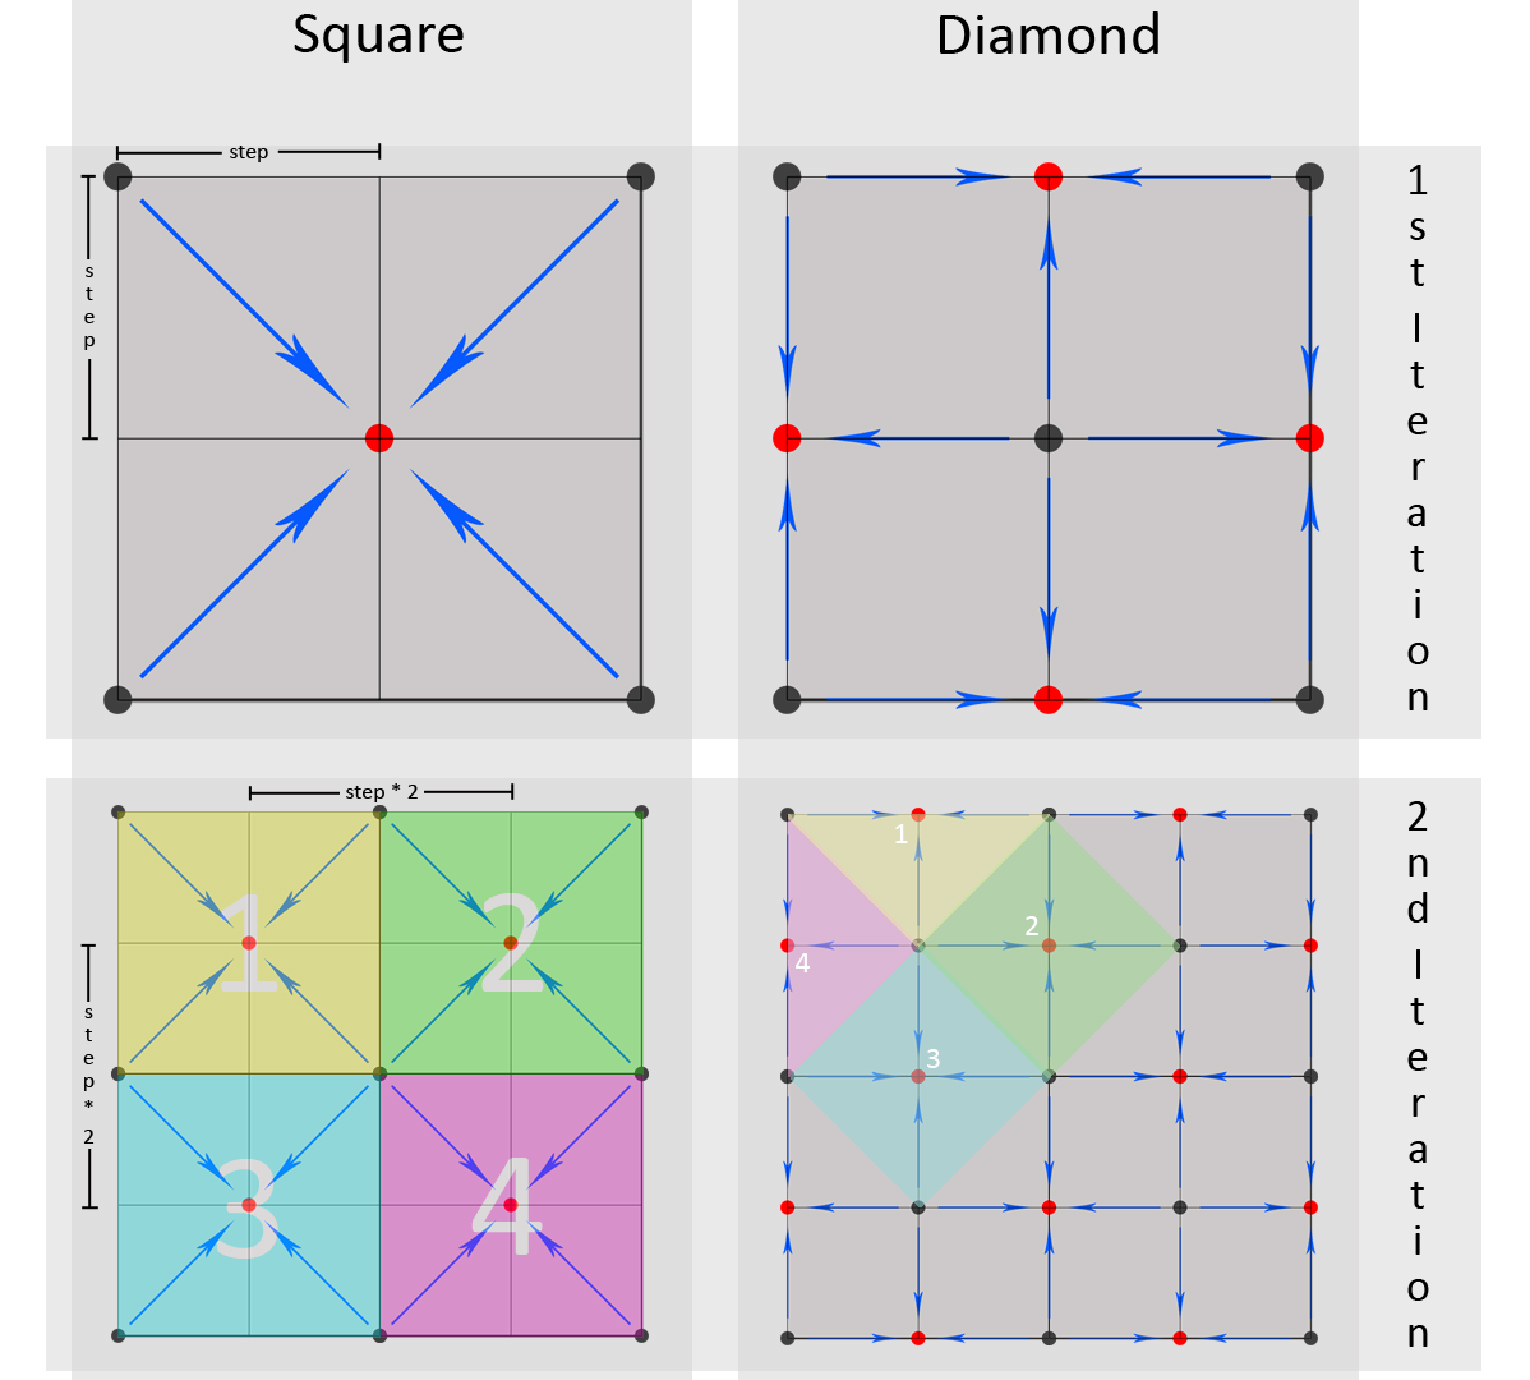
\includegraphics[width=0.4\linewidth]{images/diamondsquare.jpg}
	\caption[]{The process of the Diamond Square algorithm can be seen clearly here. }
	Image sourced from:\url{https://cmcbain.com/2014/07/31/}\\\url{procedural-terrain-generation-diamond-square-algorithm/}
	\label{fig:3}
\end{figure} 


The second is the variation parameter, $h$, which dictates how the world varies with respect to each iteration. Without a variable $h$, each iteration is free to vary from the last by whatever maximum height limit is set, however by reducing $h$ with each iteration, the smaller the square/diamond, the less the central midpoint value is allowed to deviate from its surroundings. Therefore, the variation function dictating how $h$ changes is key to how the algorithm reacts and behaves. These modifications are best seen in the pseudocode in Algorithm \ref{alg:1}.

\begin{algorithm}
\SetAlgoLined
\KwData{arrayLength, seed, startingMaximum}
\KwResult{heightMap[][]}
Generate 2D array of type double = heightMap[][]\;
Initialise random number generator with seed = randGen()\;
Set corner values of heightmap with random perturbations\;
Initialise $h$ as startingMaximum/2\;
\While{heightMap is incomplete}{
\tcp{Diamond step}
Calculate square corner average = $avg$\;
Set centre value = $avg$*h*randGen()\;
\tcp{Square step}
\If{boundary==true}{Get value from opposite side}
Calculate diamond corner average = $avg$\;
Set centre value = $avg$*h*randGen()\;
$h$ = f($h$)\;
}

\caption{The Diamond-Square Algorithm }
\label{alg:1}
\end{algorithm}

The resulting output of this produces a heightmap that can be used in conjunction with a set of tile transformation probabilities, allowing for the introduction of alternative tile types such as hills, forests, plains and mountains that occur at varying heights (see Fig. \ref{fig:4}). Such depth adds considerable complexity to the game, expanding the number of ways the game can be played.

% \begin{figure}
%   \centering
%  	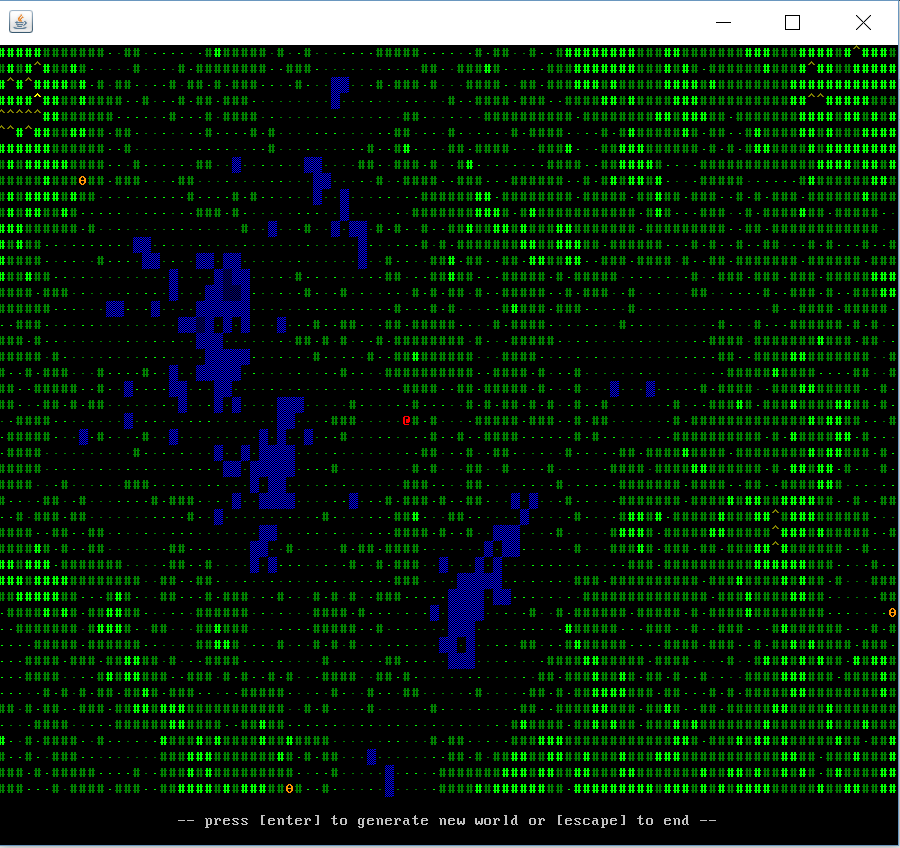
\includegraphics[width=0.4\linewidth]{images/nosmoothingendor.png}
% 	\caption[]{An example of the diamond-square heightmap transformed into overworld tiles. High and low areas can clearly be seen.}
% 	\label{fig:4}
% \end{figure} 



Another one of our deliverables was that the program should be able to produce distinctive environments by the modification of just a few parameters. This is made possible by tweaking the heightmap transformation probabilities, producing vastly different environments and changing the way the game `feels' to play. As a proof-of-concept, the program uses a use case from the \emph{Star Wars} franchise, mimicking the planetary style of multiple different planets in order to demonstrate this capability. 


\subsection{Hybridisation}

While the diamond-square algorithm produces more aesthetically pleasing and variable results than the cellular automata approach, maps still appear too disjointed to be considered `natural', and individual anomalies still occur throughout the landscape. It is clear that in order to achieve the aims of this project, there was still more work to be done in order to negate these issues. 

In an attempt to rectify this, we experimented with various values of $h$, the smoothing parameter. Modifying this made some improvement to the generated worlds (the dependence of $h$ will be discussed further in Section \ref{results}), but the biggest improvement was achieved by developing a new smoothing function inspired by the cellular automata approach, and hybridising the two methods of content generation. By taking the current ruleset of the \emph{Game of Life} and adapting it to handle multiple tile types, we were able to feed in the `tile noise' generated by the diamond-square algorithm. Tiles that neighbour multiple tile types are killed and `reborn' into the tile that most surrounds them (provided the most common tile is not itself). After performing several iterations of this smoothing technique, the resulting maps were vastly improved, as can be seen in Fig. \ref{fig:5}.

\begin{figure}
\centering
\begin{subfigure}{.4\textwidth}
  \centering
  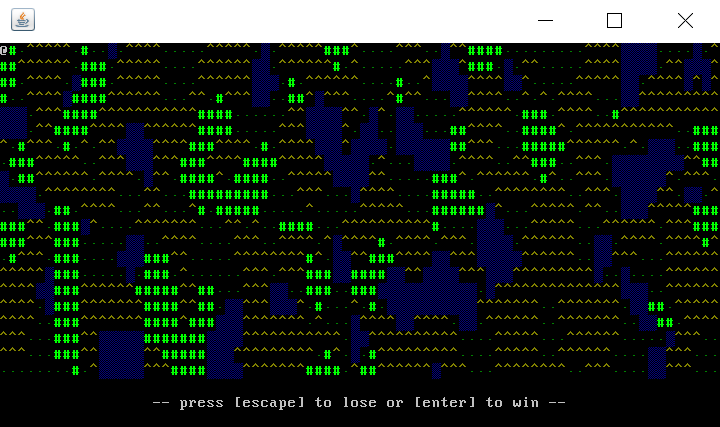
\includegraphics[width=.65\linewidth, height=3cm]{images/undersmoothing.png}
  \caption{Adapted cellular automata overworld from random noise.}
  \label{fig:4sub1}
\end{subfigure}
\hspace{20px}
\begin{subfigure}{.4\textwidth}
  \centering
  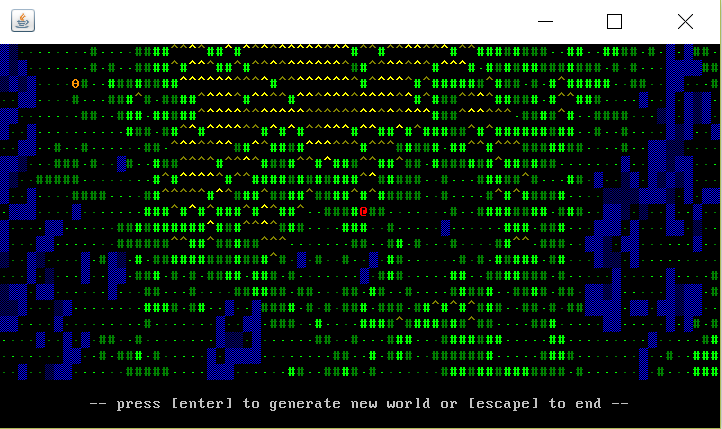
\includegraphics[width=.65\linewidth, height=3cm]{images/nosmoothingsmall.png}
  \caption{Diamond-square overworld without smoothing.}
  \label{fig:4sub2}
\end{subfigure}
\caption{A comparison of the two world generating functions can be seen here. Fig. \ref{fig:4sub2} demonstrates the contour nature of the diamond-square approach, while Fig. \ref{fig:4sub1} shows the overworld created by the adapted cellular automata algorithm with random noise.}
\label{fig:4}
\end{figure}

\begin{figure}
  \centering
 	\includegraphics[width=0.8\linewidth]{images/smoothing.png}
	\caption[]{An example of the diamond-square heightmap transformed by custom Cellular Automata smoothing function. The number of smoothing iterations is shown in each image.}
	\label{fig:5}
\end{figure} 



\subsection{Space-Filling Curves}

The results of the hybridised approach to world building look promising, with interesting features and added complexity introduced to the worlds. However our implementation is still lacking a crucial aspect of our target aims, whereby there is no predefined structure to the content that is generated. To add this element into the game we introduced a second component- caves, and sought to introduce a pre-defined structure with underlying deterministic fractal mathematical functions, such as the Hilbert curve, in a novel approach not yet seen to the best of our knowledge in previous roguelikes. 

This is achieved by taking random segments of a space-filling curve and overlaying them on top of a white noise function, which is then smoothed over by means of the existing Cellular Automata ruleset. The advantage of this is that the generated cave will be much more likely to have a structure, with defining curves, edges and paths from one edge to another (potentially linking to other generated segments), without being immediately obvious to the player and maintaining the natural look and feel of a procedurally generated dungeon, as seen in Fig. \ref{fig:6}. 

The curves are introduced to the world through an in-built \emph{Image to ASCII map} generator. This has the advantage of not requiring the curve to be built each time it is required (reducing runtime overheads) but also provides the functionality to introduce any arbitrary features to the cave system. This provides a very flexible tool to influence procedurally generated worlds in a way usually only possible through human design, while maintaining the unique nature of that procedurally generated content offers. A mock-up may be seen in Fig. \ref{fig:dragon}.

% \begin{figure}
%   \centering
%  	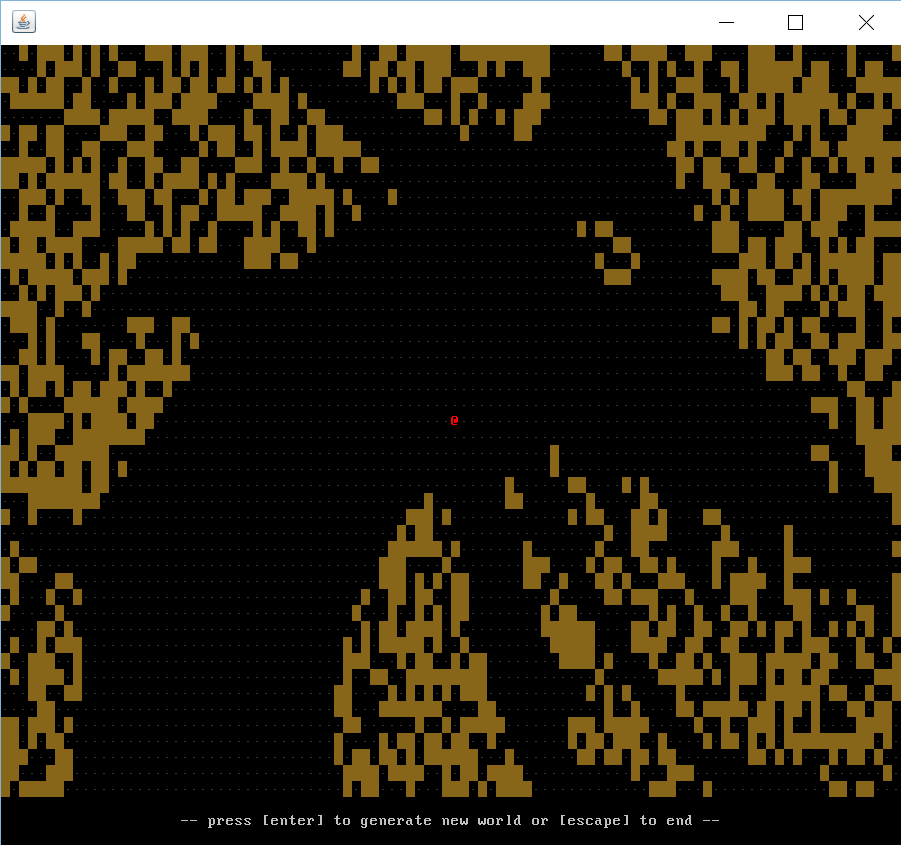
\includegraphics[width=0.3\linewidth]{images/dragonCave.PNG}
% 	\caption[]{The Hilbert curve structure can clearly be seen throughout the smoothing process, but becomes less obvious as the iterations increase.}
% 	\label{fig:dragon}
% \end{figure} 

\begin{figure}
\centering
\begin{subfigure}{.4\textwidth}
  \centering
  
\includegraphics[width=.65\linewidth, height=3cm]{images/dragon.png}
  % \caption{Adapted cellular automata overworld from random noise.}
  % \label{fig:4sub1}
\end{subfigure}
\begin{subfigure}{.4\textwidth}
  \centering
  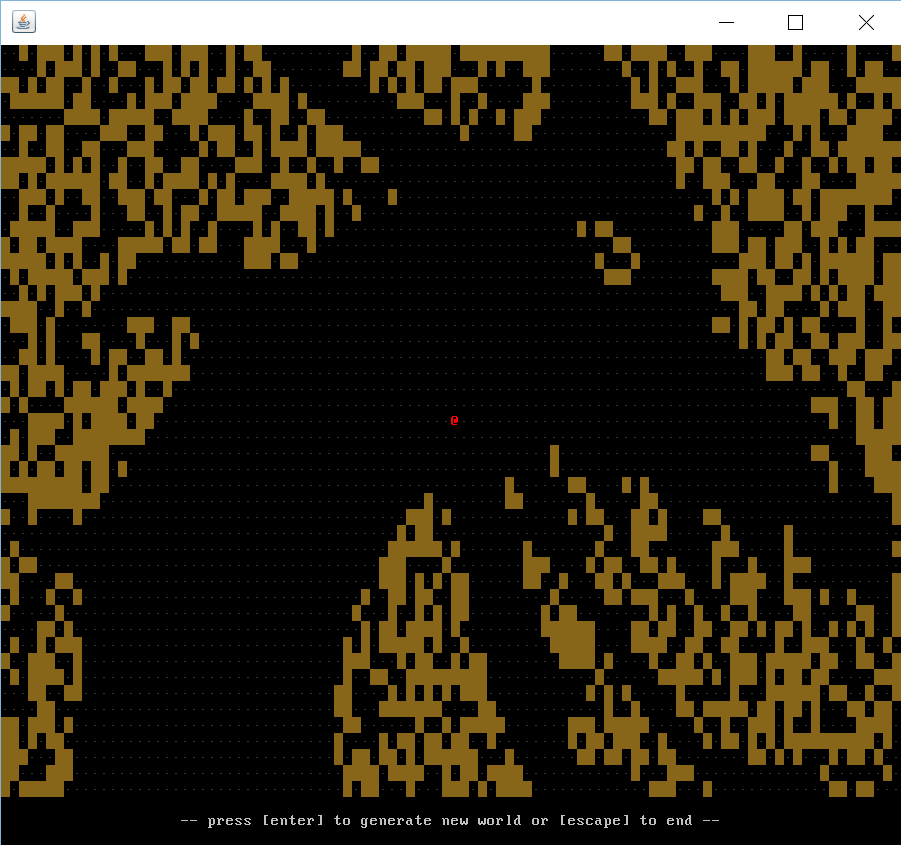
\includegraphics[width=.65\linewidth, height=3cm]{images/dragonCave.PNG}
  % \caption{Diamond-square overworld without smoothing.}
  % \label{fig:4sub2}
\end{subfigure}
\caption{The \emph{Image to ASCII map} function of the program is demonstrated here. A mock-up of a dragon can be seen. Smoothing is set to 0 here for clarity, but may be set to an arbitrary }
\label{fig:dragon}
\end{figure}


\begin{figure}
  \centering
 	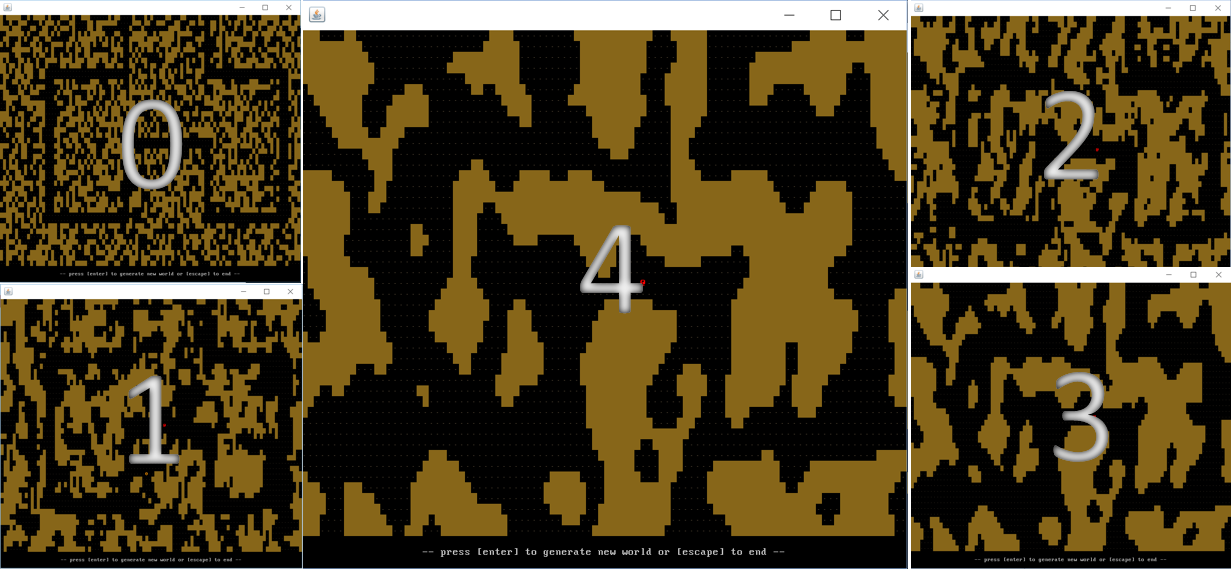
\includegraphics[width=0.8\linewidth]{images/cavesmoothing.png}
	\caption[]{The Hilbert curve structure can clearly be seen throughout the smoothing process, but becomes less obvious as the iterations increase.}
	\label{fig:6}
\end{figure} 



\subsection{Testing}

% Unit testing?
% 	- while coding, each aspect (or unit) of the program was stress tested at boundary conditions manually
% 	- final integration testing was done autonomously

% Qualatitive testing \\

% Software validation -- is carried out at the end of the system development life cycle // and was aided by the decision to use Agile methodology, since the project and product aims were assessed and then subsequently addressed in between sprints.

% Software verification-
% ensuring the program is developed according to design specifications
% Errors- were removed by unit testing, 
% Faults/Bugs 

% Bug testing- robust boundary stress testing by forcing boundary conditions \\


In order to ensure that the program we created was able to meet user requirements and was functionally and systematically stable, thorough testing was carried out. This can be split into two forms, software verification and software validation.

Verification of the program took place largely throughout the development stage of the system development life cycle (SDLC). This was in part due to the Agile nature of the development methodology, which allowed for each aspect of the program to be testing by \emph{unit} testing in-between each sprint cycle. Unit testing was also highly appropriate for this project, since the implementation language (Java) and modular software approach aligns well into specific units. This was targeted at two areas- error testing; whereby the system output was tested against the desired output, and fault testing; the checking for and correction of bugs. Fault testing was carried out using autonomous data-flow testing, such that where functions existed that required specific data inputs (such as the common occurrence of passing data in the form of 2D arrays between methods and classes), all variable cases were checked by exhaustion and the common occurrence of boundary edge checks were made by autonomously forcing array boundary conditions on all sides. At regular intervals throughout the SDLC, the program was also manually integration tested to ensure individual units worked together without fault.

Software validation was carried out at the end of the SDLC, which checked the outputs of the program against the deliverables set out at the beginning of the SDLC. Where appropriate, certain aspects of these deliverables were modified to compliment the existing capabilities of the program, while other non-functional requirements were lowered in priority as further research indicated there were better methods available. 

\subsection{Solution Pipeline}
Potential diagram of system overview

\section{Results}\label{results}


\subsection{Visualisation of Parameter Sensitivity}

The first testing strategy is purely qualitative in an attempt to describe the visual appeal of the worlds created by the algorithm. The results of several world generations may be seen in Fig. [REF], where each is achieved by changing the parameters of the algorithm. 

\begin{figure}
  \centering
 	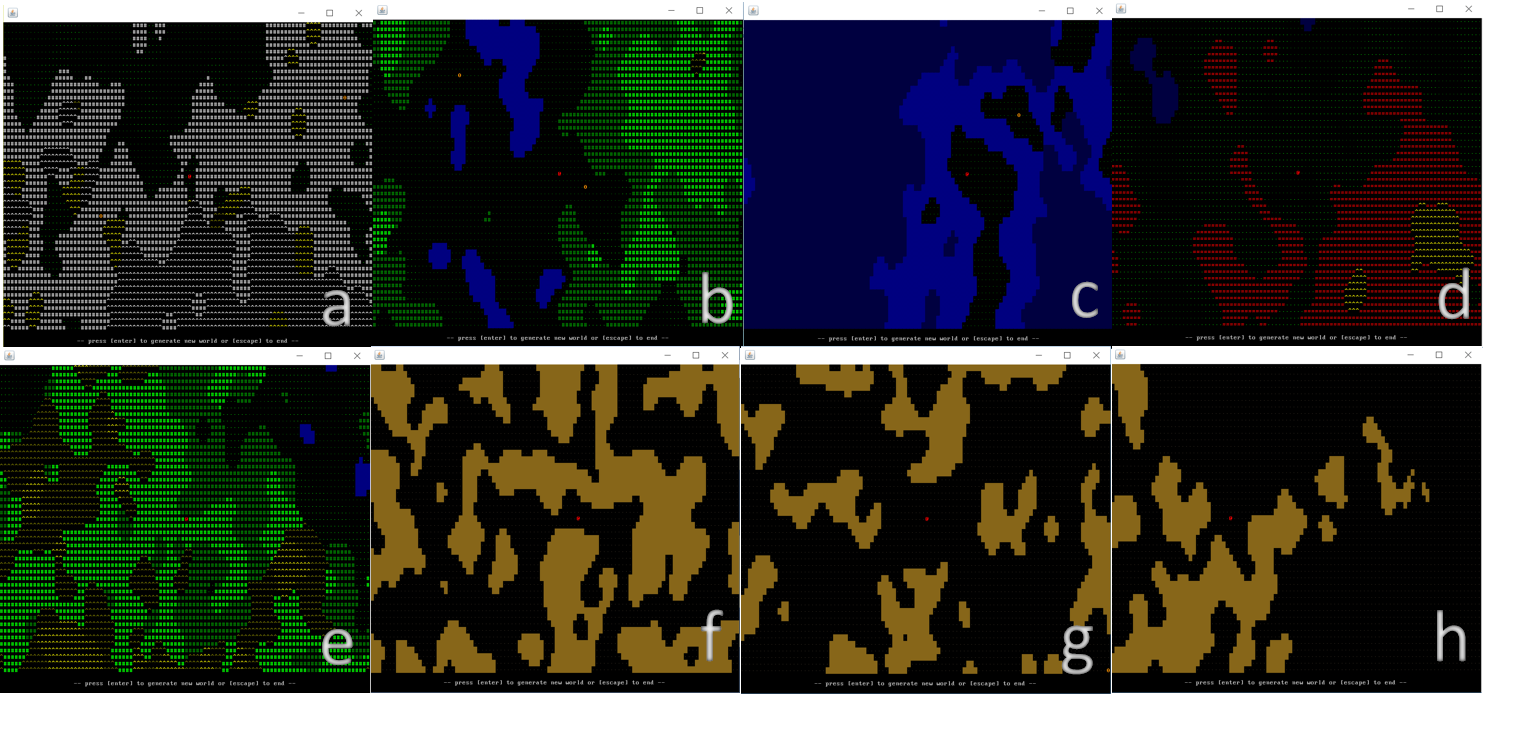
\includegraphics[width=0.8\linewidth]{images/collaboration.png}
	\caption[]{The full range of predefined outputs is displayed above. From left to right, a snowy mountainous region, a low-laying woodland, an oceanic atlantis, a fiery inferno, a chasm of valleys, a tightly bound cavern, an open and roomy cave and a hidden lost base can all be seen. Note that while these are largely proof-of-concepts, many other possibilities exist also. The images are numbered for reference.} [TOO MUCH? :-)]
	\label{fig:7}
\end{figure} 

It is clear to see that the algorithm is capable of producing worlds (such as those in Fig. \ref{fig:7}b, c and e) that match the criteria for mimicking natural landscapes well, however it is not limited to this and is also capable of recreating other fictional types of world. The cave generation is also worth mentioning- Fig. \ref{fig:7}f illustrates the aforementioned Hilbert curve but Fig. \ref{fig:7}g \& \ref{fig:7}h demonstrate different possibilities, for example the Sierpinski curve in Fig. \ref{fig:7}g generates lots of large, open spaces in cross shaped patterns. 

However while the algorithm's ability to generate vastly different environments is one of its greatest strengths, this also contributes to one of its biggest flaws (and the flaws in procedural generation as a field)- optimising the parameters to produce the `best' results is difficult and time-consuming. 

One such parameter is the diamond-square \emph{variability parameter}, $h$. Varying the function defining the parameter affects how the algorithm develops between iterations and is the secret to many well-performing algorithms. An example of different functions of $h$ with their effects on the landscape can be seen in Fig. [ref]. While many different variants of $h$ evolution functions were trialled, the five we have selected here illustrate typical examples of what can be expected from each. 

\begin{figure}
  \centering
 	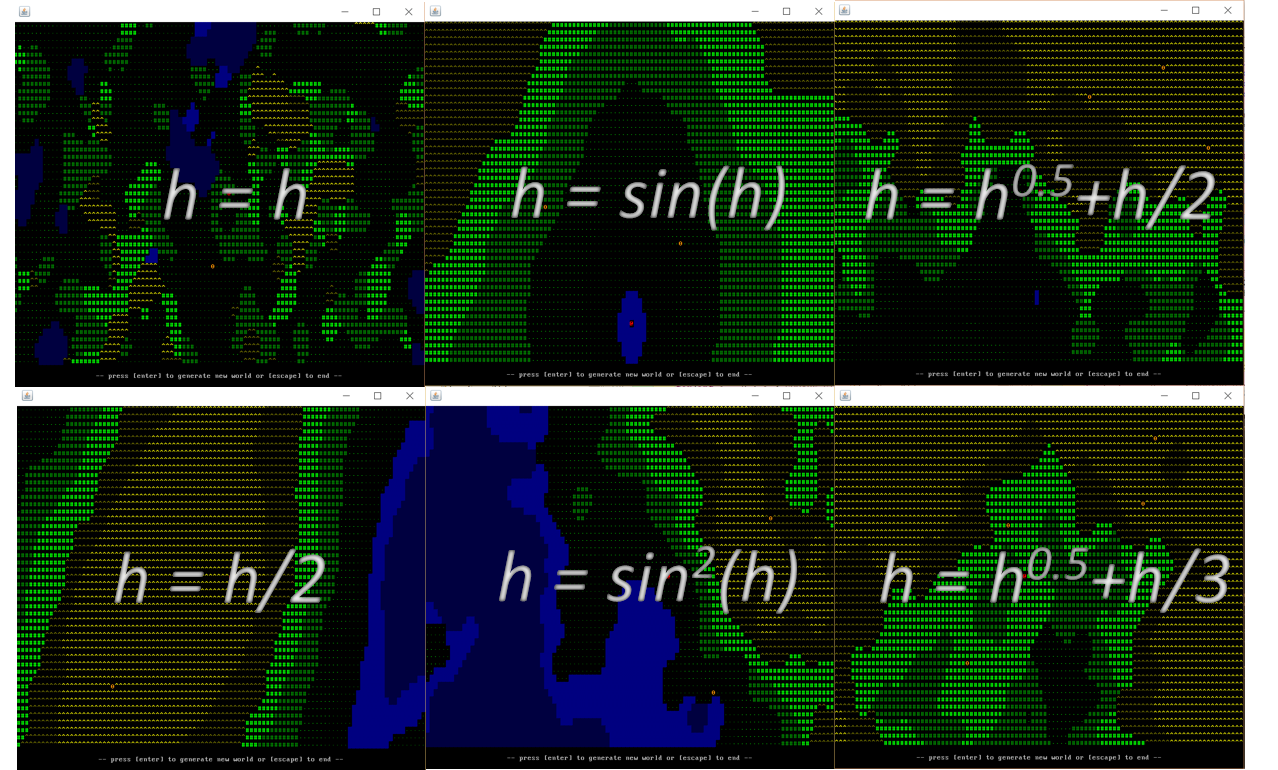
\includegraphics[width=0.8\linewidth]{images/varyingh.png}
	\caption[]{The effects of varying $h$ are shown here.}
	\label{fig:8}
\end{figure} 


It was found that the algorithm is highly sensitive to even small changes in $h$, and as such it is crucial to find the right balance between a world that varies too much, and a world that we consider too `uninteresting' to play in. In the end, we settled upon the function $h = h^\frac{2}{3} + \frac{h}{2}$, though it should be noted that while we consider this to be a good function in terms of striking a pleasant balance between a variable and naturally realistic world, this depends largely on personal preference and will be discussed further in Section [REFERENCE]. It is also interesting to note that some functions (such as $sin^2 (h)$) behave less consistently than others. We speculate that this happens because some functions converge to a low variability faster than others, while oscillatory functions such as $\sin(x)$ give rise to highly varying variability as the algorithm develops. Functions that converge quickly to a low variability coefficient are therefore highly sensitive to the initial seeding values (in the corners of the heightmap where the algorithm begins), since should these all by chance happen to be similar, terrain tends to be largely invariant across the map. By contrast, functions that do not converge quickly can give rise to particularly variable maps, especially if the corner seeding values happen to be largely different.     

% In an attempt to understand the behaviour of different functions of $h$ and their effects on the generated world, we have plotted 


To increase the consistency of created worlds, we attempted to generate a world fitness heuristic, capable of assessing created worlds on-the-fly and discarding those deemed below the threshold set. This however proved challenging, and entire fields of study exist based around the topic \cite{togelius2011search}. The result of this was the introduction of the \emph{variance parameter}, $v$, which was post-generation calculated based upon the statistical standard deviation of the resultant heightmap. Arguing that worlds below a set standard deviation would be deemed too invariant by the average player, 

We argue that worlds with a low variability are likely to be less interesting for a player to play. However too much variability (shown in Fig. \ref{fig:8}) may also lead to gameplay complications and detract from the natural feel of the game. To solve this problem, we calculate the standard deviation of a given heightmap and are able to discard worlds that fall outside of a given range, providing the player with a new world. This worked moderately well, however certain maps still experienced high diversity in some areas, while local groups of largely invariant terrain plagued other areas. This lead to the secondary introduction of the \emph{maximum feature count}, which also scrapped maps exhibiting large areas of invariant terrain while showing some diversity in other areas. It should be noted that these parameters are variable, and randomly fluctuate between pre-defined values depending on the seed, still allowing for variation between the in-game worlds. Different world biomes also exhibit this behaviour, for example the fiery world in Fig. \ref{fig:7} is deliberately more variable, breaking up the in-game world and providing the potential for more difficult in-game gameplay. 

A final parameter that we assess in each world is the \emph{openness} parameter, or connectedness coefficient. This is dependant on the players starting location, and seeks to calculate how much of a world the player is able to access from their current location. Should the player be unable to access above a specified percentage of the world (dependant on the world type), the player is moved somewhere different and the parameter is calculated again. Should no sufficient place be found after 10 attempts, the player is placed in the best possible location given those tested by the computer. This in turn enhances the playability of the game, and is implemented with a breadth-first search of the players immediate surrounding area following a random player placement. 

\subsection{Time Complexity}

An important part of procedural content generation assessment is the speed and efficiency of the algorithm created. Fast algorithms allow for in-game evaluation and redrawing of algorithms- the faster an algorithm is to run, the more stringent success criteria may be set. Additionally, fast algorithms provide good scalability, with implications in fields such as MMOGs where large maps are a requirement. To provide a comprehensive assessment of the speed of the world creation algorithm, the world creation method has been evaluated 200 times for a varying value of $z$, the square width of the map. The results can be seen in Fig. \ref{fig:9}, both for the world creation algorithm (the combination of Cellular Automata and the diamond-square algorithm), and for the breadth-first search based player placement algorithm.  


\begin{figure}
  \centering
 	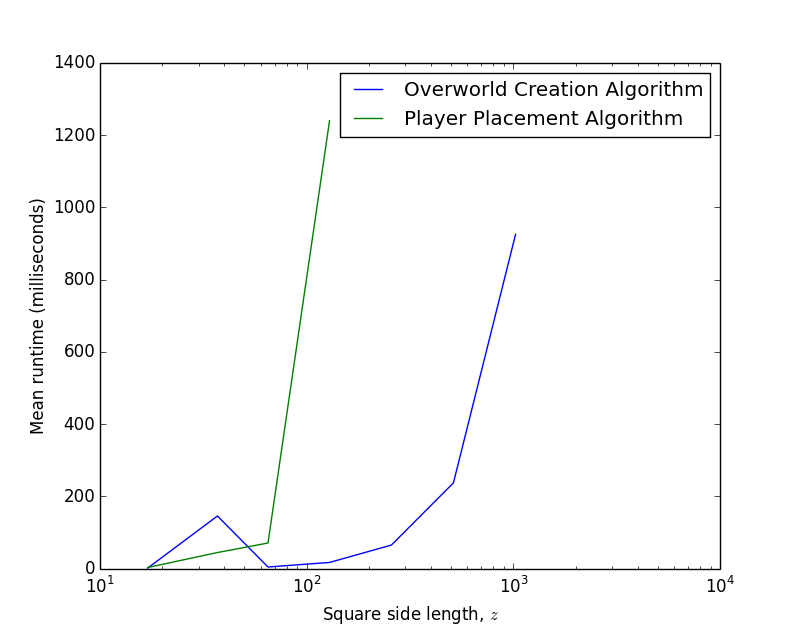
\includegraphics[width=0.5\linewidth]{images/speedtest.png}
	\caption[]{The speed of each algorithm is compared with the square side length, $z$. The mean runtime was calculated after running the world simulation 200 times, and the player placement simulation 50 times for each square side length.}
	\label{fig:9}
\end{figure} 

The tests were carried out on a moderately powerful computer with an i7 processor clocked at 4 $\times$ 2.4 GHz [NECESSARY?]. The world creation algorithm can be seen here running remarkably quickly, with an average runtime of just 4.84 milliseconds for worlds of a `standard' size at 129x129, and appears to scale as factor of $z^2$ with increasing map width. This is in agreement with the theoretical time complexity of order O($z^2$) for the diamond-square and cellular automata algorithms. The player placement algorithm however, based on a breadth-first `flood-fill' search, is much slower, and appears to scale with a time complexity exponential to an increasing square length side. This is much slower than its predicted time complexity of O($z^2$) (linear with increasing nodes), and likely owes to an inefficiency in the design implementation. Further to this, the player placement algorithm calls a breadth-first search up to 10 times in different in-game locations before the best position is selected, compounding the time-complexity of the algorithm. An interesting feature to note is the spike in mean runtime at a square side length of $z$ = 37. After inspection, this is due to the maximum world feature coefficient being consistently breached at this side length, causing the algorithm to scrap and rebuild the world up to 8 times before returning the best. The conclusion of this data shows that while the world building algorithm scales very well to increasing world sizes (less than a second evaluation time for worlds of over 1,000,000 tiles), further optimisation of the breadth first search is required. In addition to this, a local search or a different algorithm (such as Djikstra's concurrent search algorithm) should be considered for larger world sizes. Since this is not the primary aim of this work, an exhaustive breadth-first search suffices as a proof-of-concept.


\section{Evaluation}

% Appraisal of project organisation- what? \\




We now reflect upon the original research problem whereby we ask `can we improve upon existing methods of procedurally generated content in roguelike games'. We answer this question by evaluating the strengths and limitations of our proposed solution. 

\subsection{Suitability of Approach}

The first design aspect of the software was based around project enablers- these include the selected programming language and software development methodology. In hindsight, Java alongside the Eclipse IDE has proved to be an excellent design choice, permitting the use of multiple libraries to improve the project development cycle and providing a robust framework for the project to build around. The Agile methodology however, had both benefits and negatives that should be considered in future work. Rapid sprint cycles complimented the modular nature of the project, but building an early prototype and then progressing with increasingly added complexity put strain on the system and caused a number of unexpected bugs. This was compounded by the development of new ideas and approaches that came to light during the development stages of the project, for example the introduction of an overworld/cave system lended well to the 2 algorithms strengths, but required a number of classes to be modified and rewritten in places to enable the concurrent nature of multiple game environments. 

\subsection{Strengths} 

This work can report great success from aspects of the project and in general was able to meet many of its deliverables to a high standard. The world building algorithm created takes two popular approaches and combines them, enabling the production of vastly different, distinctive and aesthetically pleasing worlds. It also is the first roguelike world-building algorithm to the best of our knowledge to combine the use of random noise and world smoothing with deterministic space-filling curves, which are used to great effect in player accessible caves. Furthermore, the program is capable of bridging the gap between procedurally generated content and manual feature creation by the use of its image conversion tool, which seeds underlying noise functions with prominent custom shapes to provide unique experiences within a roguelike setting. 

Additionally, we succeeded in our goal to implement an algorithm with fast runtime overheads, and the highly efficient nature of the content generation approach not only allows the creation of vast roguelike world environments, but also makes it relevant in other related fields that require a highly scalable content generation approach. Furthermore, an efficient runtime also enables the use of in-game world screening methods. Certain aspects of these were implemented well, for example the rejection of worlds that were overpopulated by a certain tile, and the rejection of worlds who's standard deviation was too great or too low, however there remains some scope for improvement- described below. 

Another aim of the project was to implement and incorporate the use of space-filling curves. This is one of the greatest successes of the project and its potential to define underlying structure to otherwise chaotic worlds negates one of the largest difficulties with using procedurally generated content- that the created worlds may be unsuitable for player progression. Further to this, the implementation allows the introduction of any image to be used to create dungeon content. This bridges the gap between PCG and manual content creation methods, and could be used to add procedurally generated elements to otherwise manually created environments in roguelike games and farther afield. 


\subsection{Limitations}

While there are many advantages to the methods described in this work, there are a few drawbacks that should be considered. The first of these is that the algorithms described are highly sensitive to their input parameters. While this is one of the great strengths of PCG (the concept that by changing a few probabilities, vastly different outputs can be created), getting these parameters `right', such as the variability function $h$, or the tile transformation probabilities (governing which heightmap values translate to which tiles), is a challenging and time-consuming process. A potential solution to this problem would be the development of a complete world evaluation heuristic, capable of calculating the quality of generated worlds while subtly altering the input parameters- feeding back the highest scoring of these to the programmer during the alpha testing phase. In this work we attempted to create a world evaluation heuristic for the purpose of autonomously screening poorly scoring worlds, and while we had some success in this front as mentioned in the above, we were only able to evaluate worlds based on a few criteria: global height variability and maximum feature counts. Other potential features of such a heuristic might include local variability, completeness, the existence of suitable areas to place monsters/items, among others. 
% These could be achieved in a variety of ways

Another limitation of the program is the inefficiency of the breadth-first search implemented to check the suitability of the players starting location. This impacted on the runtime of the program and may be improved in future work to reduce runtime overheads, however perhaps a better and more scalable approach would be to estimate the connectivity of a section instead. This could be achieved by means of an A* search or concurrent Dijkstra's algorithm, or by terminating after a certain required number of nodes had been explored. 

\subsection{Discussion of Techniques}

As mentioned this work makes good use of the diamond-square fractal algorithm for noise generation. This was primarily selected for its ability to create contour-based heightmaps and its fast evaluation speed, however other methods were also considered and more popular methods exist throughout the industry \cite{pgcbook}. One of these is the Perlin noise algorithm, invented by Ken Perlin in 1985 \cite{imagesynth}. This method of noise generation is widely used in fields such as computer graphics \cite{textmodel}, and is generated by the combination of multiple noise images at varying resolutions and interpolating across the combination to produce a complex heightmap. While we considered this approach in the design development phase of our work, we argue that the higher resolution noise images created by Perlin noise would be unnecessary in a roguelike game environment, and the more efficient \cite{surveyPNF} diamond-square algorithm was selected instead. 

In this work we evaluate how successful a world is based on how interesting a world is to play, and how pleasing the world looks aesthetically. These are difficult factors to judge, and so parameters were chosen based on how natural the results looked, how variable the terrain generated was and how much of the world a player could access. Striking a balance between the two was judged by eye with the aid of statistical analysis in the form of heightmap mean and standard deviation, however both former evaluation criteria are subjective to the player's personal preferences. In this way, judging the success of the current selected parameters would have benefited from \emph{user evaluation testing}. Since this work however is a proof-of-concept and is aimed at the development and implementation of different algorithms (as opposed to an anthropological study of how those are interpreted by a user), the subjective fine-tuning of the world-building parameters was deemed outside of the scope of this project. [NOTE UNCONVINCED OF THE WORDING HERE]


\subsection{Conclusion}

The importance of this work can be expressed by the quality of its results and its contributions to the field of study. To summarise our solution, we have created two methods of generating procedurally generated worlds within a roguelike game environment. The first of these combines a fractal diamond-square noise algorithm with a modified version of Cellular Automata in order to create interesting and natural overworlds, and the latter combines binary white noise with Cellular Automata and mathematical space filling curves in a novel approach not before seen in roguelike games. We use this to demonstrate not only the power of procedural generation, but the potential uses of combining these methods to give procedurally generated content structure and purpose within a roguelike setting. 

The introduction of mathematical functions to general noise algorithms efficiently solves a common problem in procedural content generation where content can be criticised for lacking structure, and the success of this approach in our work may also be relevant not only to other roguelike games, but in wider gaming industry also where procedural generation techniques are used without guarantee of a set path for the player to embark on.   

Furthermore, with our inbuilt image integration function, we are able to blend both the benefits of manual content creation with procedural techniques, producing character in roguelike worlds that is difficult to achieve with traditional procedural methods.

One of the biggest problems with relying on pseudo-random number generators in games to create content compared with traditional methods is that there is no guarantee that the created content is of a sufficient quality to interest a player \cite{risi2014automatically}. Here, we address this problem by calculating statistical data about a heightmap of a given world in order to deduce conclusions about its variability, and our highly efficient implementation enables us to autonomously regenerate worlds that do not conform to our strict world criteria- ensuring a certain standard of world is passed to the player. 

One avenue for further work would be to further quantitatively identify features of a given world that make it appealing to the player, and incorporate these into a larger world heuristic function in order to further ensure the quality of a given world. Current work by Linden, Lopes and Bidarra, 2013, attempts a similar approach in a different context by using designer-expressed constraints in a \emph{generative graph grammar}; specifying actions that they wish the player to be able to make before evaluating generated worlds on their ability to achieve this. Additional further work might look at comparing the outputs of the diamond-square noise algorithm described in this work with the outputs from alternative noise algorithms (such as Perlin noise), and drawing comparisons to see whether any correlation exists between said algorithms and designer-expressed world constraints.   




% - square worlds only , tweaking or tiling of the algorithm would be necessary
% - its possible to generate its own space filling curves 


% Strengths:\\
% Produces excellent visual worlds most of the time\\
% Ability to introduce arbitrary features inside caves from ASCII graphics \\
% Very fast to generate worlds \\


% Limitations:\\
% Slow breadth first search\\
% Only capable of doing square maps currently\\
% Doesnt generate space filling curves by itself \\
% Could report more statistical information to describe and shape worlds \\
% Ability to add underlying ASCII only in caves \\

% - Talk about software enablers 
% 	- Java (SE 1.8)
% 	- Reiterate why java was chosen from design report 
% 	- talk about the prevalence of libraries 
% 	- abstraction 
% - platform neutral 
% - familiarity 

% 	look at the 3d canyon paper for a good example
% 	include psuedocode here for the diamond square algorithm and cellular automata 
% - Reinstate the aims

% \section{Questions: } 

% When to use \emph{Cellular Automata} or `Cellular Automata'
% Psuedocode improvements? \\
% References:\\
% -too many urls?\\
% -unnecessarily takes up lots of space currently \\
% Linebreaks between paragraphs? \\
% Image URL sources, shorten to goo.gl/asdfgh ?\\
% Introduction- Shift some content to related work? \\
% Related work:\\
% -roguelikes or wider context? \\
% -Introduce perlin noise here? then talk about in evaluation why not used?\\

% Concerned about lack of formal evaluative measures -> low marks for large sections





% \renewcommand{\bibfont}{\footnotesize}
% \RaggedRight
\bibliography{bib}{} %Accesses bib.bib bibliography file

\bibliographystyle{unsrt} %Makes it so the numbers are ordered correctly

\end{document}